
\Lecturer{Hui Jin}
\Contributor{}
\LectureNumber{06}
\LectureDate{DATE}
\LectureTitle{Capacity For Binary Input Memoryless Channel}

\lstset{style=mystyle}

\MakeScribeTop

%#############################################################
%#############################################################
%#############################################################
%#############################################################

\section{Introduction}
In our discussion of block linear codes, we have seen that the tradeoff between the rate of the code, ie \(R= k/n\), and the decoding error probability \(P_e\), is fundamental. On one hand, to achieve reliable communication over a noisy channel, we need to add sufficient redundancy as a funciton of the noise level; on the other hand, the redundancy added reduces the actual information that can be transmitted over. So what is this optimal trade-off, as a function of the noise level present in the communication channel? Since noise is stochastic, we have to state the problem carefully. 

Before Shannon’s 1948 work, people generally assumed that getting reliable communication, i.e. driving the bit error rate \(P_b \rightarrow 0\) requires a vanishing rate. But Shannon in his landmark 1948 paper showed that we do not have to sacrifice rate to communicate reliably. 

\paragraph{Shannon's limit} Shannon’s remarkable theorem on channel coding gives a definitive answer on this trade-off. The theorem identifies when reliable transmission is possible over the stochastic noise models. In particular, for the general framework of noise models, Shannon defined the notion of capacity \(C\), which is a real number such that reliable communication is possible if and only if the rate is less than the capacity of the channel. 

In other words, given a noisy channel with capacity \(C\), if information is transmitted at rate \(R\) for any \(R < C\) , then there exists a coding scheme that guarantees negligible error probability of communication. On the other hand if \(R > C\), then regardless of the chosen coding scheme there will be some message for which the decoding error probability is bounded from below by some constant. 

In this chapter, we will review some of the fundamental concepts in information theory, in the context of a communication channel with noise. We discuss these concepts more relevant to the channel coding: entropy, relative entropy, and mutual information. Then we define the channel capacity, aka Shannon's limit, as the maximum mutual information over the input probability function. For simplicity, we focus on binary input memoryless channels. Then, we will describe the channel capacity for some of the standard binary input noise models. Finally we state Shannon’s theorem, and show a sketch of the proof for the special case of Binary Symmetric Channel.

\section{Information Theory}
\subsection{Entropy Of A Discrete Random Variable}
Suppose \(X\) is a discrete random variable over a finite support set \(\mathcal{X} = \{x_1, x_2, \cdots, x_n\}\). Let \(p_i = P(X=x_i)\) for each \(1 \leq i \leq n\). The entropy of \(X\) is defined as 
\begin{align}
    H(X) = \sum_{x \in \mathcal{X}} p(x) \log \frac{1}{p(x)} = \sum_{i=1}^{n} p_i \log \frac{1}{p_i}.\label{eq:entropy}
\end{align}
We can use any base in the log in the above definition. If we use log in base \(2\), the resulting unit of the entropy is bit; if we use the natural log, then the unit is nat. In our discussion, we use log in base \(2)\) as the default.

The entropy \(H(X)\) of a discrete random variable \(X\) is a measure of the amount of uncertainty associated with the value of \(X\) given its density function. The more uniform the distribution is, the higher the entropy.



\begin{example}
Let \(X\) represents the outcome of a single coin toss of a fair coin. Then \(\mathcal{X} = \{H, T\}\) and \(p_1 = p_2 = \frac{1}{2}\). We have \(H(X) = 1\) bits. 
\end{example}

\begin{example}
    Let \(X\) represents the outcome of a single coin toss of a biased coin, where the probability of getting a head is \(p\) and the probability of get a tail is \(1-p\). Here \[H(X) = -p\log_{2} p - (1-p) \log_{2} (1-p) = H(p)\] bits. 

    The graph of the function \(H(p)\) is shown in Figure~. The figure illustrates some of the basic properties of entropy: first, it is a concave function of \(p\), and it is symmetric, and the uncertainty is maximum when \(p=\frac{1}{2}.\)
\end{example}

\begin{example}
Let \(X\) represents the outcome of a single roll of a fair die. Then \(\mathcal{X} = \{1, 2, 3, 4, 5, 6\}\) and \(p_i = \frac{1}{6}\) for each \(1\leq i \leq 6\). Here we have \(H(X)= \log_{2}(6)\) bits.
\end{example}

\begin{theorem}
Assume \(X\) is a discrete random variable over a finite support set \(\mathcal{X} = \{x_1, x_2, \cdots, x_n\}\). Then 
\[ 0 \leq H(X) \leq \log n.\]
Furthermore, \(H(X)=0\) iff \(p_i=1\) for some \(i\); \(H(X)=\log (n)\) iff \(p_i = 1/n\) for all \(i\).
\end{theorem}

\textbf{Proof:} First in the definition of entropy Eq~\ref{eq:entropy}, each term \(p_i \log \frac{1}{p_i}\) is non-negative, so \(H(x) \geq 0\). Since term \(p_i \log \frac{1}{p_i}\) is zero iff \(p_i = 0\) or \(1\), we have \(H(X)=0\) iff \(p_i=1\) for some \(i\).

For the other direction, we use the fact that \(\log\) function is concave down and apply Jensen's inequality:
\begin{align*}
    H(X) &= \sum_{i=1}^{n} p_i \log \frac{1}{p_i} \\
        &\leq \log (\sum_{i=1}^{n}p_i \frac{1}{p_i}) \\
        &= \log(n).
\end{align*}
For Jensen's inequality to hold equality, all \(p_i\) must be equivalent, which equals to \(\frac{1}{n}\).

\subsection{Joint Entropy}
We now extend the entropy definition to a pair of random variables \(X, Y\). If we treat the pair of random variable \((X,Y)\) as a new random variable \(Z=(X,Y)\), which is a Cartesian product of two random variables, then the entropy of \(Z\) is the joint entropy of the two random variables \(X,\) and \(Y\).

\begin{definition}
    The joint entropy \(H(X,Y)\) of a pair of discrete random variable \(X,Y\) with a joint distribution \(p(x,y)\) is defined as 
    \[ H(X,Y) = -E[\log p(x,y)] = -\sum_{x,y} p(x,y) \log p(x, y).\]
\end{definition}

\begin{theorem}
If \(X, Y\) are two independent random variables, ie \(p(x,y) = p(x)p(y)\), then 
\[H(X,Y) = H(X) + H(Y).\]
\end{theorem}

\subsection{Conditional Entropy} 
The conditional entropy of \(Y\) given \(X\) is defined as
\begin{equation}
H(X|Y) = - E[\log {p(x|y)}] = - \sum_{x \in \mathcal{X}, y \in \mathcal{Y}} p(x,y) \log_{2} p(x|y), \label{eq:CondEntropy}
\end{equation}
where \(\mathcal{X}\) and \(\mathcal{Y}\) denote the support sets of \(X\) and \(Y\). 

Another way to think about \(H(X|Y)\) is to treat \(H(X|Y=y)\) as a random value and \(H(X|Y)\) is the expected value of this random variable. 

\begin{equation}
H(X|Y) = E_y[H(X|Y=y)] = \sum_{y \in \mathcal{Y}} p(x,y) \log_{2} p(x|y), \label{eq:CondEntropy2}
\end{equation}


We will verify that this view gives the same value as the official definition. 


\begin{theorem} (Chain rule)
\begin{equation}
    H(X,Y) = H(X) + H(Y|X).
\end{equation}
\end{theorem}

\begin{proof}
Fundamentally this follows from the well known relationship:
\begin{equation*}
p(x,y) = p(x)p(y|x).
\end{equation*}

Taking logarithm both side, we have 

\begin{align*}
-\log p(x,y) = -\log p(x) - \log p(y|x).
\end{align*}

Therefore, 
\begin{align*}
    H(X,Y) &= - \sum_{x,y} p(x,y) \log p(x,y) \\
           &= - \sum_{x,y} p(x,y) \log p(x) - \sum_{x,y} p(x,y) \log p(y|x)  \\
           &= H(X) + H(Y|X)
\end{align*}

\end{proof}


\subsection{Relative Entropy} 

Entropy of a random variable is a measure of the amount of the information required on the average to describe the random variable; it is a measure of the distribution. 

Relative entropy or Kullback Leibler divergence is a measure of the distance between two distributions \(p(x)\) and \(q(x)\)


\begin{definition}
\begin{equation*}
D(p||q) = \sum_{x} p(x) \log \frac{p(x)}{q(x)}.    
\end{equation*}
\end{definition}

Using relative entropy as a target function is an important technique in machine learning. For example, in image classification, we minimize the the relative entropy between the estimated probability density function and the labeled data density function. 


\subsection{Mutual Information}
The mutual information (MI) of two random variables is a measure of the mutual dependence between the two variables. 

It is defined as
\begin{align}
I(X,Y) &= H(X) - H(X|Y)
\end{align}

In plain language, \(H(X)\) is the uncertainty for the random variable \(X\), \(H(X|Y)\) is the uncertainty for the random variable \(X\) after \(Y\) is known, so \(H(X) - H(X|Y)\) is the information about \(X\) contained in the \(Y\), or the mutual dependence.


Alternatively, the mutual information can be defined as a relative entropy between two distributions on \(X,Y\): the joint density \(p(x,y)\) and the product of the marginal distribution \(p(x)p(y)\).

\begin{definition}
Let \((X,Y)\) be random variables over alphabet \(\Sigma_X, \Sigma_Y\). If the joint distribution is \(p(x, y)\), and the product marginal distribution is \(p(x)p(y)\), then mutual information is the Kullback-Liebler Divergence of \(p(x,y)\) and \(p(x)p(y)\), ie
\begin{equation}
    I(X;Y) = D_{KL}(p(x,y)||p(x)p(y)) = \sum_{x\in\Sigma_X}\sum_{y\in \Sigma_Y} p(x,y) \log \frac{p(x,y)}{p(x)p(y)}
\end{equation}    
\end{definition}

We can show that this definition is consistent with the first definition. 

\begin{proof}
\begin{align*}
    D_{KL}(p(x,y)||p(x)p(y)) &= \sum_{x\in\Sigma_X}\sum_{y\in \Sigma_Y} p(x,y) \log \frac{p(x,y)}{p(x)p(y)} \\
    &= - \sum_{x\in\Sigma_X} \sum_{y\in \Sigma_Y} p(x,y) \log p(x) - \sum_{x\in\Sigma_X} \sum_{y\in \Sigma_Y} p(x,y) \log \frac{p(x|y)} \\
    &= H(X) - H(X|Y)
\end{align*}
    
\end{proof}


The mutual information has the following properties:

\begin{proposition}
Non-negativity: ie \(I(X;Y) \geq 0\).     
\end{proposition}
\begin{proof}
    By Jensen's inequality:
    \begin{align*}
      I(X;Y) &=  \sum_{x\in\Sigma_X}\sum_{y\in \Sigma_Y} p(x,y) \log \frac{p(x,y)}{p(x)p(y)}\\
             &= - \sum_{x\in\Sigma_X}\sum_{y\in \Sigma_Y} p(x,y) \log \frac{p(x)p(y)}{p(x,y)}\\
             &\geq - \log (\sum_{x\in\Sigma_X}\sum_{y\in \Sigma_Y} p(x,y) \frac{p(x)p(y)}{p(x,y)} ) \\
             &= -\log (\sum_{x\in\Sigma_X}\sum_{y\in \Sigma_Y} p(x)p(y) \\
             &= -\log(1) \\
             &= 0  
    \end{align*}
\end{proof}

\begin{proposition}
Symmetry: ie \(I(X;Y) = I(Y;X)\).    
\end{proposition}
\begin{proof}
    In the second definition, the function is symmetric on \(x,\) and \(y\). So \(I(X;Y)=I(Y;X)\). That means 
    \[H(X) - H(X|Y) = H(Y) - H(Y|X).\]
\end{proof}


\subsection{The Venn Diagram of Entropy and Mutual Information}
The relationship between \(H(X), H(Y), H(X,Y), H(X|Y), H(Y|X)\) and \(I(X,Y)\) is expressed in a Venn diagram. 

\begin{figure}[h]
    \centering
    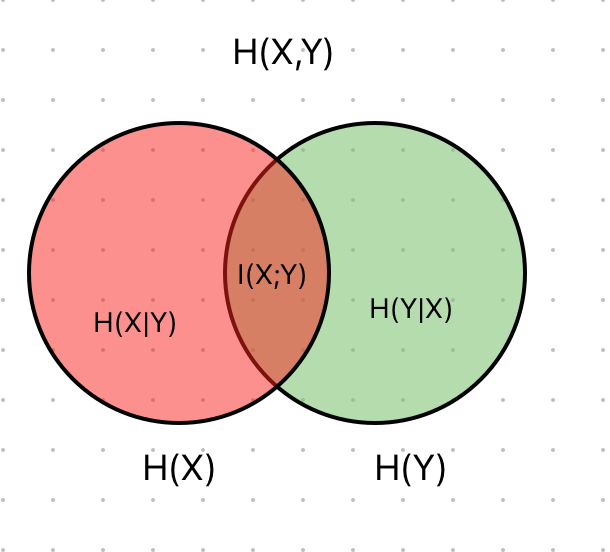
\includegraphics[width=0.6\textwidth]{Figs/Entropy_Venn.png}
    \caption{Relationship between entropy and mutual information}
    \label{fig:accumulator}
\end{figure}


\section{Capacity for Binary Input Memoryless Channels}
With entropy, joint entropy, relative entropy, conditional entropy, and mutual information defined, we are now to describe the important result of this chapter: channel capacity. Channel capacity defines the absolute upper limit for channel coding: in 1948, Shannon showed that no matter how clever we are, the channel codes have to operate below the channel capacity to achieve reliable communication. Equally astonishingly, Shannon showed that if the rate is below the channel capacity, then reliable communication is absolutely possible!

We will not give the full proof of this result in a general setting. Instead, we will give a short summary on the channel capacity of various binary input memoryless channels, describe the channel coding theorem, and prove one part of it.

\subsection{Channel Capacity}
\begin{definition}
    Channel Capacity: this is the maximal rate of reliable communication:
    \begin{align*}
        C = \sup{R| R \mbox{ is achievable}}
    \end{align*}
\end{definition}

\begin{theorem}
The channel capacity equals to the maximum mutual information.
\[C = \sup_{p_{X}(x)} I(X;Y).\]
where the supremum is taken over all possible choices of \(p_X(x)\).        
\end{theorem}

This is profound because it relates how much we can physically transmit over a channel reliably to the mutual information between input and output. This makes the complicated problem of finding channel capacity a clean optimization problem which involves finding the input distribution that maximizes the mutual information between the input and the output.

Let us state the Noisy-channel coding theorem in a formal way.
\paragraph{Noisy-channel coding theorem}
\begin{theorem}
The noisy-channel coding theorem states that for any error probability \(\epsilon > 0\) and for any transmission rate \(R\) less than the channel capacity \(C\), there is an encoding and decoding scheme transmitting data at rate R whose error probability is less than \(\epsilon\), for a sufficiently large block length. Also, for any rate greater than the channel capacity, the probability of error at the receiver goes to \(0.5\) as the block length goes to infinity.
\end{theorem}

\subsection{Noiseless Binary Channel}
Let us assume a channel whose binary input is reproduced exactly at the output. 

\begin{align*}
    C &= \max I(X;Y) \\
      &= \max H(Y) - H(Y|X) \\
      &= \max H(X) \\
      &= 1
\end{align*}
which is achieved by using \(p(x) = \{\frac{1}{2}, \frac{1}{2}\). 

\subsection{Binary Symmetric Channel}
The binary symmetric channel has symmetric crossover probability \(p\).

\begin{align*}
C = \max I(X;Y) \\
  &= \max H(Y) - H(Y|X) \\
  &= \max H(Y) - H(p) \\
  &\leq 1 - H(p)  
\end{align*}
this is achievable when \(p(x) = \{\frac{1}{2}, \frac{1}{2}\), when \(p(y=0) = p(y=1) = \frac{1}{2}\).
So the channel capacity of BSC is \(1-H(p).\) 

\subsection{Binary Erasure Channel}
In the binary erasure channel, a fraction \(p\) of the bits are erased and the received knows the location of the erasures. So the received bits can be \(01*0111\star01\cdot\), where \(star\) represents the erasures and the non-erasures are received correctly. 
\begin{figure}[h]
    \centering
    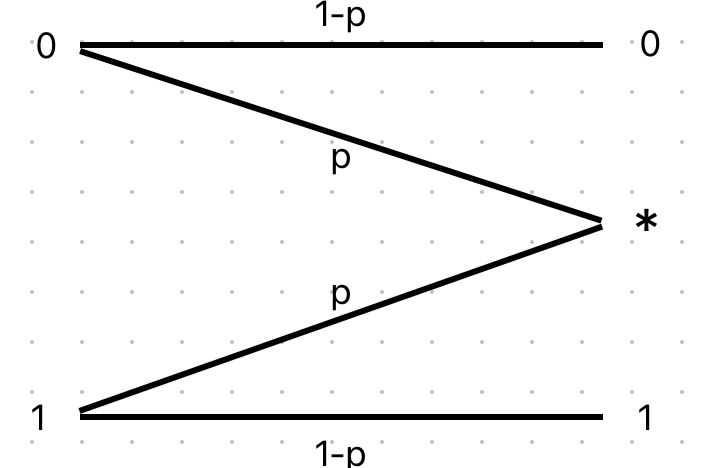
\includegraphics[width=0.5\textwidth]{Figs/BEC_channel.png}
    \caption{Binary Erasure channel. A bit has probability \(p\) erased; otherwise, it is received correctly. BEC is a good model for internet traffic.}
    \label{fig:accumulator}
\end{figure}

\begin{align*}
C = \max I(X;Y) \\
  &= \max H(Y) - H(Y|X) \\
  &= \max H(Y) - H(p) 
\end{align*}

Now assume \(p(x= 0) = \pi,\) then \(p(x=1) = 1- \pi\), and we have \(p(y=0) = \pi (1-p), \), \(p(y=1) = (1-\pi) (1-p), \) and \(p(y=\star)= p.\)
So 
\begin{align*}
    & H(Y) \\
    &= - \pi (1-p) \log (\pi (1-p)) - (1-\pi) (1-p) \log ((1-\pi) (1-p)) - p \log p \\
    &= (1-p)(-\pi \log (\pi) - (1-\pi)  \log (1-\pi)) - (1-p) \log (1-p)(\pi + (1-\pi))  - p \log p\\
         &= (1-p) H(\pi) + H(p). 
\end{align*}

Therefore \(C= \max H(Y) - H(p) = \max (1-p) H(\pi) = 1-p, \) where the maximum is achieved at \(\pi = \frac{1}{2}.\)

This being the upper limit for channel coding on the binary erasure channel makes intuitive sense: since the channel erases fraction \(p\) of the transmitted bits, the total redundancy we increase has to be at least \(p\) to have a change at reliable communication, otherwise what received is smaller than the intended information. So the code rate has to be less than \(1-p.\) 


\subsection{Binary input Additive White-Guassian-Noise Channel}
The Binary Additive White-Gaussian-Noise Channel (abbreviated as BAWGNC) is often used as a practical model in many digital communication schemes (such as transmission of data over a pair of wires). In practice, many types of noise sources are additive and independent of each other and thus, when added together, can be approximated by a zero-mean Gaussian random variable with some variance, say \(\sigma^2\). This approximation is justified by the central limit theorem.

The BAWGNC(\(\sigma)\) channel, as depicted in Figure 1, accepts a realization of a random variable \(X \in \{-1, +1\}\) on its input and outputs a realization of a random variable \(Y = X + Z\), where \(Z\) is a zero-mean Gaussian random variable with variance \(\sigma^2\). When combined together, we obtain the following conditional pdfs of Y
This channel is fully described by the noise variance \(\sigma^2\).

The capacity of this channel is given by the following formula

\[C_{BAWGN}(\sigma) = - \int_{-\inf}^{\inf} \Phi(y, \sigma) \log_2 \Phi(y, \sigma) dy - \frac{1}{2} \log_2 (2\pi \exp \sigma^2), \]

where \(\Phi(y, \sigma\) is a mixtured Guassian: 
\[\Phi(y, \sigma) = \frac{1}{2\sqrt{2\pi \sigma^2}} (\exp[-\frac{(y-1)^2}{2\sigma^2}] + \exp[-\frac{(y+1)^2}{2\sigma^2}]) \]

The derivation of this formula is beyond the scope of this class as it requires differential entropy. Interested students can find it in "Elements of Information Theory" by T. Cover and J. Thomas. 
\section{Channel Coding Theorem}
\begin{theorem}
For any error probability \(\epsilon > 0\) and for any transmission rate \(R\) less than the channel capacity \(C\), there is an encoding and decoding scheme transmitting data at rate R whose error probability is less than \(\epsilon\), for a sufficiently large block length. Also, for any rate greater than the channel capacity, the probability of error at the receiver goes to \(0.5\) as the block length goes to infinity.
\end{theorem}

\paragraph{Achievable Region}
Graphs for BSC, BEC, and AWGN will be included here. 

BSC: 1- H(p)
BEC: 1- p
AWGN: 

\subsection{A Sketch of the Proof of the Channel Capacity}
The channel capacity theorem states that if and only if the code rate is below the Shannon's limit, reliable channel coding scheme is feasible.  

At the heart of the proof is the typical set idea: given transmitted codeword \(c\), what received typically resides inside a shell of a sphere.

\subsubsection{Typical set}
Let us consider a transmitted codeword \(c\). The received message \(y\) will differ from \(c\) at \(pn\) positions with increasingly high probability; in fact, the probability that 
\[Pr(|d(y, c) - pn| > \epsilon) < \exp( - \epsilon^3 /n) \]
by Chernov's bound. That means for each transmitted codeword, the received vector is most likely with Hamming distance \(pn\) from the codeword, or we can say it resides in a shell around the codeword with radius \(pn\).  We call this is the typical set \(T_{p}(c)\) around codeword \(c\).

\subsubsection{If \(R > C\), then error probability is bounded away from \(0\)}
Here, we are going to prove one direction of the channel capacity theorem: if the code rate \(R\) is above the channel capacity, then it is impossible to achieve arbitrarily small error probability for at least some of the transmitted codewords. 

We actually can prove a stronger result. If the rate \(R\) is above the channel capacity, then the decoding error probability for some codeword has to be at least \(1/2\). 

The basic idea is: if the decoding error probability for a codeword is less than \(\frac{1}{2}\), then for the typical received vector, at least half of them should be in the decoding sphere around the codeword. So the volume of this sphere has to be large. That means we cannot pack too many such spheres, or too many codewords, into the linear space of \(2^n\). That gives the limit of the code rate.    



For reliable communication, these shells around codewords should be decoded correctly for at least half of them to achieve error rate less than \(\frac{1}{2}\).  


Let us first estimate the volume of each of these spheres. We need the Stirling's formula to approximate the factorials in the binomial expansion:  
\[n! = \sqrt{2\pi n} (\frac{n}{e})^n (1 + o(n)).\]

Since the sphere's volume is lower bounded by the half of the shell of distance \(pn\), we have
\begin{align*}
V_0 &\geq \frac{1}{2} \binom{n}{pn} \\
    &= p^{-pn}(1-p)^{-(1-p)n} (1 + o(n)) \\
    &= 2^{H(p)n - o(n)}
\end{align*}

This actually gives a physical interpretation of the entropy function: It represents the volume of the sphere around the codeword.  

Now consider totally how many codewords we can pack there with the constraint that these correct decoding regions do not overlap. This can be easily bounded: 
\begin{align*}
2^k V_0 &< 2^n \\
2^k 2^{H(p)n -o(n)} &< 2^n \\
k + H(p) n - o(n) &< n \\
R = k/n &< 1-H(p) - \epsilon 
\end{align*}
for any arbitrarily small $\epsilon$. In other words, if the code rate is above the Shannon's limit, then reliable communication is infeasible. 

\subsubsection{Typical Pairs Decoding}
Our decoding algorithm will be: if there is a unique codeword \(c\) within distance \((p + \delta)n\) from
the received word \(y\), decode to \(c\). Otherwise, give up. We will show that this works with high
probability.

\subsubsection{If \(R < C\), then error probability goes to \(0\) as \(n\) goes large}

If \(R < C\), then the total number of codewords is \(|C| = 2^{Rn} \leq 2^{(1-H(p)-\epsilon)n}.\)

What is the probability that our received word is not decoded properly? First, with probability
\(1− \epsilon\), the received word is close enough to the original codeword \(c\). In this case, the only reason
for the decoding to fail is if another codeword is also within \((p + \delta)n\) distance from the received
codeword. 

We will compute the probability that our received word is decoded to a specific other
codeword \(c^{'}\). Recall that the codewords were chosen at random. Thus, the probability that a
specific codeword \(c\) is within distance \((p + \delta)n\) from our received word \(y\) is exactly the probability
that a random binary string is within distance this of \(c^{'}\). This is just the ratio of the number of
words close to \(c^{'}\) to the total number of words, or approximately
\[\frac{2^{n H(p)}}{2^n} = 2^{-(1-H(p))n}.\]

Then by the union bound, the error probability that the typical pairs decoding makes an error is upper bounded by:
\begin{align*}
    P_{E} \leq |C| 2^{-(1-H(p))n} < 2^{-\epsilon n} 
\end{align*}
which goes to zero as \(n\) goes to infinity.